\documentclass[
  10pt, % Fontsize
  a4paper, % papersize
  twoside, % For twosided documents
  openright, % Chapters start always at a odd page
  numbers=noenddot, % No final dots in Sectionnumbers, e.g 1.2 instead of 1.2.
  BCOR=5mm, % Correction length for lost space from binding
  parskip=half*, %No indent but spacing between paragraphs
  thesis, % type of document
  %ngerman, % For language setting, translations package does not see if
  % the language is set here.??
  %english,
  %french,
]{bfhbook}


% Test Template for bfhbook.cls
\usepackage[T1]{fontenc}
% Coding 
\usepackage[utf8]{inputenc}
% Language setting
\usepackage[ngerman]{babel}

% For more sophisticated blindtext, including lists, math text, etc.
\usepackage{blindtext}

% \usepackage{fonttable}
% Hyperref
\usepackage[                
  pdftex,                  % for PDF
  colorlinks=true,         % colored links
  linkcolor=black,         % color for links
  citecolor=black,         % color for references
  urlcolor=black,          % color for url 
  bookmarks=true
]{hyperref}              

\usepackage[acronym,toc]{glossaries} % Generate Glossaries
\usepackage{booktabs} % For nicer tables
\usepackage{threeparttable} % Table-Captions having the same width than the table
\usepackage[singlelinecheck=off]{caption}
\usepackage{siunitx} % Scientific Units and number setting
\usepackage{listings} % For Program-Code
\usepackage{makeidx} % indexing
\usepackage[backend=bibtex,style=ieee]{biblatex}
\bibliography{mybib}

%%%%%%%%%%%%%%%%%%%%%%%%%%%%%%%%%%%
% Settings 
%%%%%%%%%%%%%%%%%%%%%%%%%%%%%%%%
% Type?? (Lecture Notes, BSc Thesis, Master Thesis, . . .) 
% Use Variables \BSc, \Master, etc. for language support
\type{Bachelor-Thesis}
% Author(s)
\author{Fabian Wittwer}
% Title
\title{Title}
% Short Title, will be used in the footline
\shorttitle{Shorttitle}
% Subtitle
\subtitle{Subtitle}
% Titlepicture
\titlepicture{elektronik.jpg}
%%

% Topic of Study
\degreeprogramme{Elektro- und Informationstechnologie}
% Supervisor
\thesisadvisor{Prof.~Dr.~I.~Newton}
% Client
\projectpartner{Google}
% Expert
\expert{A.~Einstein}
% Version
\version{1.0}
% Date
\date{\today} % Or any other possible date
% Departement
% Use Variable for language support
%\TI

% Semester
% Use Variable for language support
%\semester

% Logo(s)

% Colors
% Secondary Color for Graphics, Tables etc.
% Naming: BFH*Light|Medium|Dark*Color, e.g. BFHDarkGreen, BFHLightBlue, etc.
% Possible Color Values: Green, Blue, Purple, Brown 
\newcommand{\seccolor}{BFHLightGreen} 

\newcommand{\Tel}[2]{Tel: (#1): #2}

\setcounter{secnumdepth}{4}
\setcounter{tocdepth}{4}

\makeindex
\makeglossaries

\begin{document}
\maketitle

%**************************************************************************
\frontmatter % preliminary parts
%**************************************************************************
% Allows breaks in Math Formulars
\allowdisplaybreaks

\tableofcontents

\sloppy
%%%%%%%%%%%%%%%%%%%%%%%%
% Introduction
%**************************************************************************
\mainmatter % The main part
%**************************************************************************
%\part{Part One}
\chapter*{Management Summary}
\chapter{Einleitung}
\section{Text mit Absätzen}
Hier einige Zitate: \cite{Einstein1923}, \cite{NS87a}, \cite{SH96}.

{\Large \textbf{Schriftart ist \testfont}}

\Blindtext
\section{Text mit mathematischen Formeln}
\blindmathpaper

Beispiele für\index{Hello} Programmlistings:

Matlab:
\lstinputlisting[language=Matlab,caption={Beispiel Matlab-Code}]{listing_matlab.m}

Dasselbe Listing mit dem listings-Paket
\lstset{language=C}
\begin{lstlisting}
#include <iostream>

int main(int argc, char* argv[]) {
   using namespace std;
   cout << ''Hello world!'' << endl;
   return 0;
}
\end{lstlisting}

% Floating Objects
\blindtext asdf\index{Guggus}
\Tel{mobil}{079 123 45 67}


% Example for a Table in BFH-Style with a simple Design
\begin{table}[ht]
\renewcommand{\arraystretch}{2} % In order to set the correct linespacing.
% Must be set here, since this also changes the linespacing for the array
% environment
\arrayrulecolor{white}
	\begin{center}
		\rowcolors{1}{\seccolor!10}{\seccolor!10} % Rows with 10% of secondary color
% See page 33 of the "BFH Markenmanual"
	\begin{threeparttable}
		\caption{Anzahl Personen, ausländischer Bevölkerungsanteil und Arbeitslosenquote pro
		Stadtteil Ende 2005 (Statistikdienste der Stadt Bern, 2006)}
	\begin{tabular}{lll}
	%	\toprule
		\rowcolor{\seccolor!50}
		Stadtteil & Anzahl Personen & Ausländische
		Bevölkerung\\\bfhmidline
		Innere Stadt & \num{3748} & \SI{17.9}{\percent}\\\bfhmidline
		Länggasse-Felsenau & \num{17976} & \SI{17.1}{\percent}\\\bfhmidline
		Mattenhof-Weissenbühl & \num{26895} & \SI{22.4}{\percent}\\\bfhmidline
		Kirchenfeld-Schlosshalde & \num{23384} & \SI{13.4}{\percent}\\\bfhmidline
		Breitenrain-Lorraine & \num{24082} & \SI{19.4}{\percent}\\
		%\bottomrule
	\end{tabular}
	\end{threeparttable}
	\label{tab:tab1}
	\end{center}
\end{table}

%
\section{Section}
\blindtext
\blindtext
\begin{figure}[htp]
  \begin{center}
    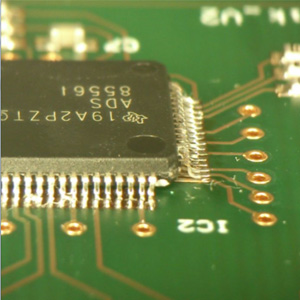
\includegraphics[width=10cm]{elektronik.jpg}
  \end{center}
    \caption{Ein Testbild}
  \label{fig:test1}
\end{figure}
Erklärender\index{fig} Text für die Abbildung \ref{fig:test1}. Mit
Fussnotentest\footnote{Fussnote!}

\blindtext
\subsection{SubsecTitle}
\subsubsection{SubsubsecTitle}
\blindtext

% Longer Documemt with chapter, sections, etc. Also many examples of
% list-environments are included.
\Blinddocument
%%%%%%%%%%%%%%%%%%%%%%%%%%%%%%%%%%%%%%%%%%%%%%%%%%%%%%%%%%%%%%%%%%%%%%%
\backmatter %

% List of Figures
\listoffigures
% List of Tables
\listoftables
% Glossary
\printglossary
% Bibliography
\printbibliography

%Index
%\addcontentsline{toc}{chapter}{Index}
\printindex

% Appendices
\chapter*{Versionskontrolle}
\renewcommand{\arraystretch}{2} % In order to set the correct linespacing.
% Must be set here, since this also changes the linespacing for the array
% environment
%\arrayrulecolor{white}
\begin{center}
  \rowcolors{1}{\seccolor!10}{\seccolor!10} % Rows with 10% of secondary color
  \begin{tabular}{llll}
  \rowcolor{\seccolor!50}
   Version & Datum & Beschreibung\index{asdf} & Autor\\\bfhmidline
    0.1 & 26.02.2013 & Dokument erstellt & Peter Muster\\\bfhmidline
    0.2 & 13.03.2013 & Dokument überarbeitet & Anna Meier\\\bfhmidline
    1.0 & 21.05.2013 & Dokument fertiggestellt & Peter Muster
  \end{tabular}
\end{center}
\end{document}
